\section{How to Make Lots of Mistakes} \label{sec:mutate}

An important challenge from section~\ref{sec:challenges} is the generation of
mix-typed programs with representative impedance mismatches between
the typed components, their types, and the behavior of untyped components. In this section, we
present a generation process and argue that, despite its synthetic
nature, it yields a large corpus of programs with  realistic and diverse type mistakes.

The starting point for our corpus of programs
is~\citet{gtnffvf-jfp-2019}'s gradual typing benchmark suite. The
benchmark suite consists of fully typed correct programs that are written by different authors
and have been used, maintained and evolved by their authors and others over a
number of years.  They range widely in size, complexity, purpose and
features of Typed Racket they employ.  Furthermore the benchmarks use advanced aspects
of Typed Racket's type system such as occurrence
typing~\cite{tf-icfp-2010}, types for mutable and immutable data
structures, polymorphic types, types for first-class classes and objects and types for
Racket's numeric tower~\cite{stathff-padl-12}. Without loss of the diversity of the benchmarks,
we select the ten largest in terms of numbers of components (between 6 and 14 components).
These benchmarks also have the most complex dependency graphs and, hence,
can make the debugging process the hardest for the rational programmer.
The table in figure~\ref{table:benchmark-descriptions} shows our selection
together with a short description for each benchmark.


\begin{figure*}
\begin{tabular}{p{2cm} | p{10cm} }
  {\bf  name} & {\bf description (author)}  \\

\hline

  \texttt{acquire} & Board game simulation (M. Felleisen)  \\%[1em]


\hline
  \texttt{gregor} & Utilities for calendar dates (J. Zeppieri) \\%[1em]


\hline
  \texttt{kcfa} & Functional implementation of 2CFA for the lambda calculus (M. Might) \\%[1em]


\hline
  \texttt{quadT} & Converter from S-expresion source code to PDF format (M. Butterick)\\%[1em]

\hline
  \texttt{quadU} & Converter from S-expresion source code to PDF format  (B. Greenman) \\%[1em]

\hline
  \texttt{snake} & Functional implementation of the  Snake video game (D. Van Horn) \\%[1em]

\hline
  \texttt{suffixtree} & Algorithm for common longest subsequences between strings. (D. Yoo) \\%[1em]

\hline
  \texttt{synth} & Converter of description of notes and drum beats to WAV format (V. St-Amour \& N. Toronto) \\%[1em]

\hline
  \texttt{take5} & Card game simulator (M.Felleisen)  \\%[1em]

\hline
  \texttt{tetris} & Functional implementation of Tetris (D. Van Horn) \\%[1em]


\end{tabular}
  \caption{Benchmarks summary.}
  \label{table:benchmark-descriptions}
\end{figure*}

Of course, the gradual typing benchmarks have no mistakes for the rational
programmer to debug. Therefore, we follow
~\citet{lksfd-popl-2020} and we inject bugs with mutation analysis.
A mutation is a local syntactic change of the code of a program that may
produce a bug.
\ll{Need citations for mutation}
Usually, the outcome of mutating a program
once, dubbed a mutant, can be distinguished from the original program with a test case.
The better the test suite of a program, the more mutants it can ``kill.''
Mutants that are hard to ``kill'' usually correspond to subtle programming errors, and mutation frameworks typically come with standard mutators carefully designed to create such mutants.

However, Typed Racket's gradual type system detects shallow errors, unlike those introduced by standard mutators.
Thus, we need different mutators to evaluate the rational programmer, ones which are fine-tuned to generate shallow errors.
The table in figure~\ref{table:mutation-ops} summarizes our mutators.
For each one, the table provides a short description and an example
mutation it performs. Each mutator is inspired by the more-than-a-decade
long experience of the authors making type-level mistakes in Typed Racket.
We find that these mistakes often take non-trivial effort to debug.

Most of our mutators in figure~\ref{table:mutation-ops} are self-explanatory.
The first twelve can apply to most gradually typed languages, including those with classes.
The last four mutators target distinguishing features of Typed Racket.
Specifically, \texttt{arithmetic} may replace a \texttt{+} with a \texttt{-}
in an attempt to change the type of the result of the arithmetic
operation. In Typed Racket, \texttt{+}'s result is a
\texttt{Positive-Integer} when all arguments are
\texttt{Positive-Integer}. However, the result of \texttt{-} is
\texttt{Integer}. In the same spirit, \texttt{boolean} aims to take
advantage of Typed Racket's ``truthiness.'' Finally, \texttt{negate-cond} and \texttt{force-cond}
aim to confuse occurrence typing.


\begin{figure*}
  \begin{tabular}{p{2.1cm} | p{5cm}  | p{5.5cm} }
    {\bf name} & {\bf description} & {\bf example} \\




    \texttt{constant}
& Swap a literal constant with another of the same value but different type.
& \texttt{5.6} $\rightarrow$ \texttt{5.6+0.0i} \\
\hline

    \texttt{deletion}
    & Deletes the result expression of a sequence.
    & \texttt{(begin x y z)} $\rightarrow$ \texttt{(begin x y)} \\
\hline

   \texttt{position}
 & Swaps two subexpressions.
  &  \texttt{(f a 42 "b" 0)} $\rightarrow$\texttt{(f a 42 0 "b")} \\
\hline

     \texttt{list}
    & Replaces \texttt{append} with \texttt{cons}.
    &  \begin{tabular}[t]{@{}l}
      \texttt{append} $\rightarrow$ \texttt{cons}
    \end{tabular}\\
\hline

    \texttt{top-level-id}
 & Swaps two identifiers defined in the same module.
 &\texttt{(f x 42)} $\rightarrow$ \texttt{(g x 42)}\\
\hline

    \texttt{imported-id}
 & Swaps two identifiers imported from the same module.
 &\texttt{(f x 42)} $\rightarrow$ \texttt{(g x 42)}\\
\hline

    \texttt{method-id}
 & Swaps two method identifiers.
 &\texttt{(send o f x 42)} $\rightarrow$ \texttt{(send o g x 42)}\\
\hline

    \texttt{field-id}
 & Swaps two field identifiers.
    & \begin{tabular}[t]{@{}l} \texttt{(get-field o f)} $\rightarrow$ \\
        \texttt{(get-field o g)}
      \end{tabular}\\
\hline

     \texttt{class:init}
  & Swaps values of class initializers.
   &  \begin{tabular}[t]{@{}l}
     \texttt{(new c [a 5] [b "hello"])} $\rightarrow$\\
     \texttt{(new c [a "hello"] [b 5])}\\
    \end{tabular}\\
\hline

     \texttt{class:parent}
    & Replaces the parent of classes with \texttt{object\%}.
    &  \begin{tabular}[t]{@{}l}
     \texttt{(class foo\% (super-new))} $\rightarrow$\\
     \texttt{(class object\% (super-new))}\\
    \end{tabular}\\
\hline

     \texttt{class:public}
    & Makes a public method private and vice versa.
    & \begin{tabular}[t]{@{}l}
      \texttt{(class object\%}\\
      \phantom{(d}\texttt{(define/public (m x) x))} $\rightarrow$\\
      \texttt{(class object\%}\\
      \phantom{(d}\texttt{(define/private (m x) x))}\\
    \end{tabular}\\
\hline

     \texttt{class:super}
    & Removes \texttt{super-new} calls from class definitions.
    &  \begin{tabular}[t]{@{}l}
      \texttt{(class foo\% (super-new))} $\rightarrow$\\
      \texttt{(class foo\% (void))}\\
    \end{tabular}\\
\hline


     \texttt{arithmetic}
& Swaps arithmetic operators.
    & \texttt{+} $\rightarrow$ \texttt{-} \\
\hline

     \texttt{boolean}
& Swaps \texttt{and} and \texttt{or}.
& \texttt{and} $\rightarrow$ \texttt{or} \\
\hline

     \texttt{negate-cond}
    & Negates conditional test expressions.
    &  \begin{tabular}[t]{@{}l}
      \texttt{(if (= x 0) t e)} $\rightarrow$\\
      \texttt{(if (not (= x 0)) t e)}
       \end{tabular}\\
\hline

     \texttt{force-cond}
    & Replaces conditional test expressions with \texttt{\#t}.
    &  \begin{tabular}[t]{@{}l}
      \texttt{(if (= x 0) t e)} $\rightarrow$\\
      \texttt{(if \#t t e)}
    \end{tabular}\\
\hline
\end{tabular}
  \caption{Summary of mutators.}
  \label{table:mutation-ops}
\end{figure*}


\subsection{Are these mutators good enough?}

Of course, mutators that introduce these kinds of shallow errors directly into the benchmarks do not produce bugs that are interesting from the perspective of the rational programmer.
The benchmarks are fully typed, so Typed Racket's type checker locates them immediately.
For that reason, we apply the mutators to versions of the benchmarks with some components stripped of type annotations (dubbed \emph{configurations}).
Without the annotations, the type checker may not detect the errors in these mutant configurations.
Instead, Typed Racket's gradual type system may detect the errors dynamically.
Mutant configurations that result in dynamic errors are the ideal ground to exercise the rational programmer's ability to locate errors.

Specifically, we define an \emph{interesting debugging scenario} as a mutant configuration that
\begin{enumerate}
\item would be rejected by the type checker if we restored the missing type annotations,
\item produces a dynamic error under Erasure as-is, and
\item the stacktrace of the error mentions at least three distinct components.
\end{enumerate}

The second and third criteria require a little more explanation.
The second criterion requires that the error is detectable under Erasure to ensure that it is detectable by all three semantics.
This is a direct consequence of~\citet{gfd-oopsla-2019}'s theorem that a dynamic type error under Erasure implies a dynamic type error under both Transient and Natural.
It is worth noting that this criterion excludes from consideration all scenarios where Natural or Transient can detect the bug but Erasure cannot, and thus it favors Erasure.
However, our goal here is to evaluate blame across these three semantics, and thus we focus on systems where all of them exhibit blame.


The third criterion aims to capture debugging scenarios with a specific kind of dynamic error: one produced by the interactions between typed and untyped components.
In those cases, the rational programmer may need to examine several components to locate the source of the bad interaction.
In technical terms, we conservatively approximate these scenarios by analyzing the stacktrace of the error.
If the stack trace mentions at least two components, then this is evidence of interaction between components.
We require the third component because our benchmarks come with a driver component which is present in every stacktrace.


\begin{figure*}
  \centering
  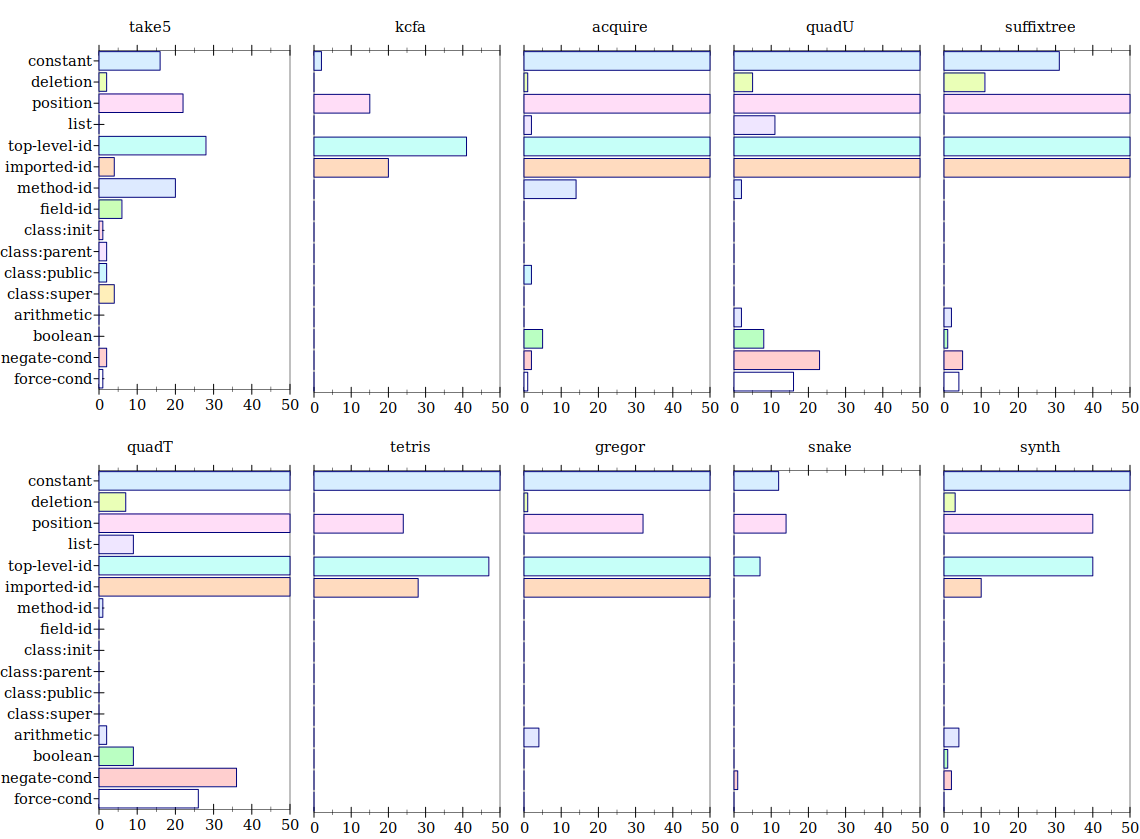
\includegraphics[scale=0.35]{./plots/mutant-breakdown}
  \caption{Interesting debugging scenarios produced by our mutators. Counts are cut off at 50.}
  \label{fig:mutant-breakdown}
\end{figure*}


With this definition in hand, we analyze how effectively our mutators produce interesting debugging scenarios from our benchmarks.
Figure~\ref{fig:mutant-breakdown} shows the number of distinct interesting debugging scenarios produced by our mutators for each benchmark.
The columns correspond to our benchmarks, and each rows show the count of interesting debugging scenarios produced by one mutator from figure~\ref{table:mutation-ops}.
The counts are cut of at 50, so any bar reaching the right side of the plot means 50 or more scenarios.

Figure~\ref{fig:mutant-breakdown} illustrates that our mutators do indeed produce a large number of interesting debugging scenarios for all of our benchmarks.
All of the mutators together produce at least 40 interesting scenarios for every benchmark, and those scenarios are produced by at least four different mutators for each benchmark.
Thus our mutators produce a large and diverse population of scenarios for every benchmark.
Furthermore, every mutator contributes scenarios to at least one benchmark.
Some mutators clearly only target one or two of them, though, and in particular the class-focused mutators are primarily effective in \texttt{take5}.
This reflects that among our benchmarks \texttt{take5} makes the most extensive use of object-oriented features, while the other features targeted by the rest of the mutators are used more broadly.
